\documentclass[11pt]{article}

\usepackage[margin=1in]{geometry}
\usepackage[T1]{fontenc}
\usepackage[utf8]{inputenc}
\usepackage{lmodern}
\usepackage{microtype}
\usepackage{amsmath,amssymb,amsfonts,mathtools,bm}
\usepackage{amsthm}
\usepackage{booktabs,array,multirow}
\usepackage{enumitem}
\usepackage{xcolor}
\usepackage{graphicx}
\usepackage{tikz}
\usetikzlibrary{arrows.meta,positioning,calc,fit,backgrounds}
\usepackage{url}
\usepackage{xurl}
\usepackage[backend=biber,style=numeric-comp,sorting=none,maxbibnames=12]{biblatex}
\addbibresource{references.bib}
\DeclareFieldFormat{url}{\href{#1}{paper link}}
\usepackage[colorlinks=true,linkcolor=blue!55!black,citecolor=blue!55!black,urlcolor=blue!60!black]{hyperref}
\usepackage[nameinlink,noabbrev]{cleveref}

\setlength{\parindent}{0pt}
\setlength{\parskip}{0.45em}
\setlist[itemize]{topsep=0.25em,itemsep=0.18em,leftmargin=1.7em}
\setlist[enumerate]{topsep=0.25em,itemsep=0.18em,leftmargin=1.8em}

\newtheorem{definition}{Definition}[section]
\newtheorem{proposition}[definition]{Proposition}
\newtheorem{lemma}[definition]{Lemma}
\newtheorem{theorem}[definition]{Theorem}
\newtheorem{corollary}[definition]{Corollary}
\newtheorem{conjecture}[definition]{Conjecture}
\newtheorem{question}[definition]{Open Question}
\theoremstyle{remark}
\newtheorem{remark}[definition]{Remark}
\newtheorem{example}[definition]{Example}

\newcommand{\indep}{\perp\!\!\!\perp}
\newcommand{\pa}{\operatorname{pa}}
\newcommand{\ch}{\operatorname{ch}}
\newcommand{\rank}{\operatorname{rank}}
\newcommand{\Tr}{\operatorname{Tr}}
\newcommand{\diag}{\operatorname{diag}}
\newcommand{\supp}{\operatorname{supp}}
\newcommand{\TN}{\operatorname{TN}}
\newcommand{\CPDAG}{\mathrm{CPDAG}}
\newcommand{\cI}{\mathcal I}
\newcommand{\cG}{\mathcal G}
\newcommand{\cT}{\mathcal T}
\newcommand{\cH}{\mathcal H}
\newcommand{\bbR}{\mathbb R}
\newcommand{\bbC}{\mathbb C}
\newcommand{\bbN}{\mathbb N}
\newcommand{\odotc}{\mathbin{\odot}}

\title{\textbf{Causal Structure and Tensor-Network Representations}\\[0.4em]\large Working Notes for a Research Program}
\author{}
\date{September 2026}

\begin{document}
\maketitle

\begin{abstract}
These working notes develop a research program at the interface of causal graphical models, tensor networks (TNs), and probabilistic machine learning. The central hypothesis is that conditional independences implied by a causal graph can be encoded by algebraic separability conditions in suitable probability-TN representations, and that the same algebraic structure can be exploited in two complementary directions. In the \emph{causal-to-tensor direction (synthesis)}, a known causal graph is compiled into a structured, learnable TN whose local tensors satisfy stochastic, copy, rank, or isometric constraints by construction. In the \emph{tensor-to-causal direction (analysis)}, a TN learned from observational data is inspected for gauge-invariant algebraic signatures from which conditional independences, v-structures, and ultimately a Markov equivalence class may be recovered.

We first formulate the program for nonnegative probability tensors, then extend it to Born models and to continuous variables represented in finite feature spaces. Particular attention is given to the difference between observable rank conditions and conditions on internal cores, the role of TN gauge freedom, positive gauges and Bayesian reparameterizations, and the special status of tree tensor networks (TTNs) and causal polytrees as a first rigorous setting. We also outline how causal algebraic structure may simplify contraction after evidence or intervention, potentially yielding a query-dependent effective contraction width. The document deliberately distinguishes established results from provisional propositions, conjectures, and open problems; it is intended as a technical basis for a future paper rather than a finished manuscript.
\end{abstract}

\tableofcontents
\newpage

\section{Introduction and research program}
\label{sec:intro}

\subsection{Motivation and central hypothesis}

A joint distribution over many variables is simultaneously a statistical object, a graphical-model object, and a high-order tensor. Causal graphical models describe which local mechanisms generate the variables and which conditional independences (CIs) follow from graph separation. Tensor networks describe high-order tensors by contracting low-order local tensors. The working hypothesis of this project is that these two forms of structure can be aligned more tightly than is normally exploited:
\begin{equation}
\boxed{
\text{causal structure}
\quad\longleftrightarrow\quad
\text{algebraic TN structure}
\quad\longleftrightarrow\quad
\text{learning and contraction complexity}.}
\label{eq:central-hypothesis}
\end{equation}

The project is not based on the claim that graphical models and TNs are unrelated formalisms: their connections are well established \cite{robeva2019duality,miller2021hybrid,ran2019bayesian}. Nor is the connection between CI and low tensor rank new: algebraic statistics, conditional probability tensor decompositions, and recent tensor-rank causal discovery methods already exploit precisely this principle \cite{molstad2026conditional,chen2024tensor,chen2025latent}. The intended contribution is more specific: to study whether causal information can be represented, learned, and queried \emph{directly in compressed TN coordinates}, and whether causal algebraic structure can become an algorithmic resource for TN learning and contraction.

A useful guiding picture is
\begin{center}
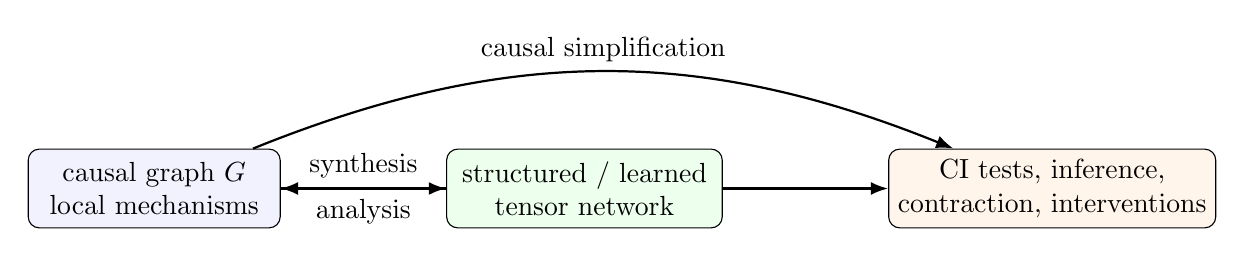
\begin{tikzpicture}[node distance=2.1cm, every node/.style={align=center}, >={Latex[length=2.2mm]}]
\node[draw,rounded corners,fill=blue!5,minimum width=3.2cm,minimum height=1.0cm] (g) {causal graph $G$\\local mechanisms};
\node[draw,rounded corners,fill=green!7,right=of g,minimum width=3.5cm,minimum height=1.0cm] (tn) {structured / learned\\tensor network};
\node[draw,rounded corners,fill=orange!8,right=of tn,minimum width=3.5cm,minimum height=1.0cm] (ops) {CI tests, inference,\\contraction, interventions};
\draw[->,thick] (g) -- node[above]{synthesis} (tn);
\draw[->,thick] (tn) -- node[below]{analysis} (g);
\draw[->,thick] (tn) -- (ops);
\draw[->,thick,bend left=22] (g) to node[above]{causal simplification} (ops);
\end{tikzpicture}
\end{center}

Two complementary research directions follow.

\paragraph{Causal-to-tensor direction (synthesis).}
Given a causal DAG $G$, construct and train a TN model $P_{\theta,G}$ whose local tensors encode the causal mechanisms and CIs of $G$ by construction. The questions are representational and algorithmic: how should conditional probability tables (CPTs) be tensorized, how can positivity and normalization be preserved, and when does evidence or intervention trigger exact algebraic splitting that reduces contraction cost?

\paragraph{Tensor-to-causal direction (analysis).}
Given samples from an unknown distribution, first learn a compressed TN $P_\theta$, then inspect gauge-invariant local or effective tensor properties to obtain a CI oracle and recover a Markov equivalence class. The central issue is identifiability: under what hypotheses must every minimal representation of the same distribution exhibit the relevant rank/separability signatures?

The first direction is currently the more mature one and is likely the natural starting point. The second is more exploratory and raises nontrivial questions about canonical forms, TN realization fibers, and the distinction between local mechanism tensors and effective tensors after contraction of the environment.

\subsection{Guiding three-variable motifs}

Let $A,X,B$ be discrete variables. A non-collider triple (chain or fork)
\begin{equation}
A\to X\to B,\qquad A\leftarrow X\to B,\qquad A\leftarrow X\leftarrow B
\end{equation}
shares the observational CI
\begin{equation}
A\indep B\mid X,
\end{equation}
whereas the collider
\begin{equation}
A\to X\leftarrow B
\end{equation}
has the generic pattern
\begin{equation}
A\indep B,\qquad A\not\indep B\mid X.
\end{equation}
For the probability tensor $T_{axb}=P(a,x,b)$, the distinction is algebraic:
\begin{align}
\text{non-collider:}\quad & \rank T_x=1\quad\forall x,\label{eq:intro-noncollider}\\
\text{collider:}\quad & \rank\!\left(\sum_x T_x\right)=1,\label{eq:intro-collider}
\end{align}
where $T_x(a,b)=T(a,x,b)$. These elementary identities will be the prototype for the more general constructions below.

\subsection{Questions currently under investigation}

The project can be organized around five increasingly difficult questions.
\begin{enumerate}
\item \textbf{Representation.} Given a DAG, which local stochastic/copy-tensor architectures realize its factorization while remaining compact and trainable?
\item \textbf{Gauge robustness.} Which causal signatures are invariant under the gauge freedom of minimal TT/TTN representations? Can changes within a Markov equivalence class be understood as positive gauge transformations, blocked gauges, or local Bayesian rewrites?
\item \textbf{Discovery.} Can CIs be tested directly from a compressed TN, avoiding explicit exponentially large contingency tensors, and can these tests be used as the CI oracle of PC-like algorithms?
\item \textbf{Computation.} Can conditioning, marginalization, or intervention expose exact rank-one factors that reduce an effective contraction graph or treewidth beyond what the original graph suggests?
\item \textbf{Extensions.} Which parts of the theory survive for Born models, continuous variables represented by finite embeddings, loopy TNs/PEPS, hidden variables, and mixed discrete--continuous data?
\end{enumerate}

\section{Background and related work}
\label{sec:background}

\subsection{Bayesian networks, causal DAGs, and Markov equivalence}

A Bayesian network on variables $X_1,\ldots,X_n$ consists of a DAG $G$ and a joint distribution satisfying
\begin{equation}
P(x_1,\ldots,x_n)=\prod_{i=1}^n P(x_i\mid x_{\pa(i)}).
\label{eq:bn-factorization}
\end{equation}
Under the causal Markov interpretation, each factor is a local mechanism and d-separation in $G$ implies CI in $P$ \cite{pearl2009causality,spirtes2000causation}. Purely observational data generally identify only a Markov equivalence class: DAGs with the same skeleton and v-structures entail the same d-separation relations. Chickering's transformational characterization shows that equivalent DAGs can be related by sequences of covered edge reversals \cite{chickering1995transformational}. This fact will later motivate a tensorial interpretation of local Bayesian rewrites.

It is important to distinguish \emph{probabilistic factorization} from \emph{causal interpretation}. Any joint distribution can be factorized according to a complete DAG by the chain rule, but that factorization does not identify the true intervention semantics. Latent confounding, feedback, selection, or an inappropriate choice of observed variables can all invalidate a naive causal interpretation of a fitted DAG. Throughout these notes, when we speak about a causal DAG we assume a structural/causal interpretation in addition to the observational factorization.

Conditioning and intervention are distinct operations. Conditioning on $X=x$ preserves the mechanism $P(X\mid \pa(X))$ and updates beliefs. The intervention $\mathrm{do}(X=x)$ replaces that mechanism by a fixed source and removes its incoming causal dependence. This distinction will have a direct TN implementation in \cref{sec:classical-general-node,sec:synthesis-rewrites}.

\subsection{Causal discovery}

Constraint-based methods such as the PC algorithm infer a skeleton by repeatedly testing statements $X_i\indep X_j\mid S$, store separating sets, orient unshielded colliders, and then propagate compelled orientations using orientation rules \cite{spirtes2000causation}. The result is a completed partially directed acyclic graph (CPDAG) representing the Markov equivalence class under causal sufficiency and standard Markov/faithfulness assumptions. Score-based methods instead search over graphs or equivalence classes. Greedy equivalence search (GES) is a canonical example \cite{chickering2002optimal}. Continuous approaches such as NOTEARS replace discrete graph search by smooth optimization over weighted adjacency matrices together with an exact differentiable acyclicity constraint \cite{zheng2018notears}.

For discrete data, CI tests commonly use contingency tables, likelihood-ratio $G^2$ tests, Pearson $\chi^2$ tests, or conditional mutual information. In Gaussian models, CI is equivalent to vanishing partial correlation. More general nonlinear continuous settings use kernel, regression, nearest-neighbor, or conditional-randomization approaches. Our proposed tensorial analysis direction does not replace causal discovery logic itself; rather, it asks whether a compressed TN can provide a new CI oracle whose complexity and statistical behavior differ from tests on raw contingency tables.

\subsection{Graphical models and tensor networks}

The relation between discrete graphical models and TNs is well established. Robeva and Seigal formalize a duality between graphical models and tensor hypernetworks, translating marginalization into contraction and relating message-passing procedures across the two formalisms \cite{robeva2019duality}. Miller, Roeder, and Bradley further develop a hybrid probabilistic graphical model--TN framework with copy/decoherence structures and discuss the relation between ordinary PGMs and Born-machine correlations \cite{miller2021hybrid}. Ran's Bayesian Tensor Network directly uses normalized nonnegative tensors as conditional probability objects in a directed acyclic TN architecture \cite{ran2019bayesian}.

For sequence models, nonnegative MPS/TT representations are closely related to hidden Markov models, predictive state representations, and weighted automata \cite{glasser2019expressive,adhikary2021quantum}. These works establish that probabilistic TNs are not merely formal encodings: they form practical and expressive statistical model classes with efficient likelihood evaluation and trainable parametrizations.

\subsection{Algebraic statistics and tensor-rank causal discovery}

For discrete variables, many CI constraints are polynomial equations. The simplest example is $A\indep B$, which is equivalent to all $2\times 2$ minors of the probability matrix vanishing. Conditional independence $A\indep B\mid X$ yields the same rank-one condition slice by slice in $x$. Molstad and Zhang exploit the relation between conditional independence and low rank of conditional probability tensors in multivariate categorical regression \cite{molstad2026conditional}.

Recent causal discovery work goes further. Chen et al. relate ranks of observed contingency tensors to separating latent-variable sets and use tensor-rank conditions to identify latent structure \cite{chen2024tensor}; subsequent work extends the approach to mixed observed data and latent confounding \cite{chen2025latent}. Consequently, ``rank tests imply causal discovery'' is not by itself a novel claim. The distinct question here is whether the same information can be extracted from a \emph{compressed learned TN} through local/effective tensor algebra, potentially without materializing the full contingency tensors on which existing rank tests operate.

\subsection{Context-specific independence, causal independence, and tractable circuits}

Boutilier et al. formalize context-specific independence (CSI), where independence holds only for particular assignments of conditioning variables, and show how such structure can improve inference through specialized CPT representations and decompositions \cite{boutilier1996context}. Heckerman and Breese study causal independence, where a many-parent mechanism admits internal functional factorization, enabling more efficient representation and inference than a generic CPT \cite{heckerman1994causal}. Both are conceptually close to our synthesis direction: local causal mechanisms may contain algebraic structure that is not visible from graph topology alone.

Probabilistic and arithmetic circuits provide another comparison point. Their tractability relies on structural properties such as decomposability and determinism, and efficient compilation can transform difficult graphical models into representations supporting particular operations \cite{shen2016tractable}. Wang and Kwiatkowska show how structured probabilistic circuits can support polynomial-time causal queries such as backdoor adjustment \cite{wang2023compositional}. Our proposed TN viewpoint can be read as a multilinear analogue: evidence may expose low-rank separability, causing a TN to become effectively decomposable for a particular query.

\subsection{Contraction complexity and algebraically tractable TNs}

TN contraction complexity depends strongly on graph width. Markov and Shi connect tensor-network simulation complexity to treewidth-type quantities \cite{markov2008simulating}, while exact contraction of generic PEPS is computationally hard \cite{schuch2007complexity}. In Bayesian networks, Chen and Darwiche's causal treewidth shows that functional/deterministic mechanism structure can yield inference complexity substantially below that suggested by ordinary treewidth \cite{chen2022causal}. This supports a broader principle relevant here: graph topology alone need not determine inference complexity when local factors have exploitable algebraic structure.

In quantum TNs, isometric constraints offer a particularly strong analogy. IsoTNS impose local isometries that cancel in double-layer contractions and make otherwise difficult two-dimensional calculations efficient \cite{zaletel2020isometric}; dual-isometric PEPS impose multiple isometric conditions and enlarge the efficiently computable class \cite{yu2024dual}. Our proposed causal constraints are different, but the computational philosophy is similar:
\begin{equation}
\text{local algebraic identity}\quad\Longrightarrow\quad\text{global contraction simplification}.
\end{equation}
Roa-Villescas et al. demonstrate the algorithmic usefulness of modern TN contraction methods for general probabilistic inference tasks \cite{roavillescas2024probabilistic}. Thus a causal-aware preprocessing or rewriting stage could potentially feed directly into state-of-the-art TN contraction pipelines.

\subsection{Gauge freedom and representation identifiability}

Different TN cores can represent the same global tensor. For fixed-rank TT manifolds, this redundancy is described by invertible changes of basis on internal bonds \cite{holtz2012manifolds}. Fundamental-theorem results for normal PEPS similarly characterize when tensors generating the same state are related by local gauges \cite{molnar2018normal}. These results motivate the central analysis question: if a distribution has a causal TN representation with local rank signatures, are all relevant minimal representations in the same gauge orbit, so that those signatures are unavoidable?

There is also a graphical-model literature on gauge reparameterizations. Ahn, Chertkov, and Shin optimize edge-local gauge transformations that alter factors while preserving the partition function \cite{ahn2017gauging}. This is not causal discovery, but it provides precedent for treating probabilistic factor reparameterization through a TN-like gauge language.

\subsection{Continuous and stochastic applications}

Functional tensor trains replace discrete TT cores by matrix-valued functions and provide a continuous analogue of TT decomposition \cite{gorodetsky2019functional}. Meiburg et al. develop generative TN models for continuous data and show how finite feature embeddings can retain efficient TN calculations while extending MPS generative modeling beyond categorical inputs \cite{meiburg2025continuous}. These ideas motivate our finite-feature-space treatment in \cref{sec:continuous}.

Classical stochastic dynamics provide natural application domains. Probabilistic cellular automata can be learned with MPOs \cite{casagrande2024pca}; MPS methods can represent full probability distributions for epidemic contact processes \cite{merbis2023epidemic}; and reaction--diffusion rare-event dynamics can be computed using TN representations of the full stochastic ensemble \cite{nicholson2023rare}. Such space--time models come with explicit local causal neighborhoods and therefore provide promising testbeds for both synthesis and causal-aware contraction.

Finally, the phrase ``causal tensor network'' already appears in quantum-process settings: J\o rgensen and Pollock exploit the causal TN structure of process tensors to simulate non-Markovian path integrals efficiently \cite{jorgensen2019causal}. Any future title should therefore make clear that our focus is causal graphical structure in probabilistic/nonnegative and Born TN models.

\section{Tensorial foundations of probabilistic causal structure}
\label{sec:foundations}

\subsection{General setting}

Let $X_1,\ldots,X_n$ be random variables. For finite alphabets $\mathcal X_i$, the joint distribution is the nonnegative tensor
\begin{equation}
T_{x_1\cdots x_n}=P(X_1=x_1,\ldots,X_n=x_n),\qquad T\ge 0,\qquad \sum_{\bm x}T_{\bm x}=1.
\end{equation}
A tensor-network representation introduces internal indices $\alpha_e$ and local cores $A^{[v]}$, such that
\begin{equation}
T_{\bm x}=\operatorname{Contr}\left(\{A^{[v]}\};\bm x\right).
\end{equation}
We distinguish three levels throughout:
\begin{enumerate}
\item the \emph{observable probability tensor} $T$;
\item an \emph{effective tensor} obtained by contracting part of the TN environment;
\item a \emph{bare local core} $A^{[v]}$ before its environment is contracted.
\end{enumerate}
Rank properties of $T$ need not be rank properties of an arbitrary overparameterized or loopy local core. Much of the analysis direction consists of identifying settings---especially minimal TT/TTN representations---where this distinction can be controlled.

\begin{definition}[Conditioning and marginalization]
For a discrete physical index $x$, conditioning on $X=x^\star$ fixes the physical leg to $x^\star$. Marginalization over $X$ contracts that leg with the all-ones covector, i.e.
\begin{equation}
T_{\mathrm{marg}}=\sum_x T_x.
\end{equation}
These two operations should not be confused with intervention, which modifies the causal mechanism itself; see \cref{sec:interventions-foundation}.
\end{definition}

\subsection{Classical nonnegative tensor networks}
\label{sec:classical}

\subsubsection{Three-variable prototype}

Consider
\begin{equation}
T_{axb}=P(A=a,X=x,B=b),
\end{equation}
and define the matrix slice $T_x\in\bbR_{\ge0}^{d_A\times d_B}$ by
\begin{equation}
[T_x]_{ab}=T_{axb}.
\end{equation}

\begin{proposition}[Conditional independence as slice rank]
\label{prop:classical-slice-rank}
On the support where $P(X=x)>0$,
\begin{equation}
A\indep B\mid X
\quad\Longleftrightarrow\quad
\rank T_x=1\quad\text{for every }x.
\end{equation}
\end{proposition}
\begin{proof}
If $A\indep B\mid X$, then
\begin{equation}
T_x(a,b)=P(x)P(a\mid x)P(b\mid x),
\end{equation}
which is an outer product. Conversely, any nonnegative rank-one slice can be normalized into the product of its row and column marginals, yielding the corresponding conditional independence.
\end{proof}

\begin{proposition}[Marginal independence as rank]
\label{prop:classical-marginal-rank}
\begin{equation}
A\indep B
\quad\Longleftrightarrow\quad
\rank\!\left(\sum_x T_x\right)=1.
\end{equation}
\end{proposition}

The chain and fork motifs therefore share the slice-rank signature of \cref{prop:classical-slice-rank}, while a generic collider has the marginal-rank signature of \cref{prop:classical-marginal-rank} but not the slice-rank signature.

\subsubsection{Explicit local forms for chains, forks, and colliders}

For a non-collider triple, a local tensor can be written as
\begin{equation}
B_{\alpha x\beta}=u_{\alpha x}v_{x\beta}.
\label{eq:classical-chain-form}
\end{equation}
Equivalently,
\begin{equation}
B=\sum_x u_x\otimes e_x\otimes v_x,
\end{equation}
so every physical slice is rank one. The vectors $u_x$ and $v_x$ absorb arbitrary nonnegative weights, including a factor $P(x)$ distributed between the two sides.

For a collider, a useful exact local form is
\begin{equation}
B_{\alpha x\beta}=a_\alpha b_\beta Q(x\mid \alpha,\beta),
\qquad
Q(x\mid\alpha,\beta)\ge0,
\qquad
\sum_xQ(x\mid\alpha,\beta)=1.
\label{eq:classical-collider-form}
\end{equation}
Then
\begin{equation}
\sum_xB_{\alpha x\beta}=a_\alpha b_\beta,
\end{equation}
so marginalizing the collider physical variable produces rank one across the left--right partition, whereas a fixed-$x$ slice can have arbitrary rank through $Q(x\mid\alpha,\beta)$.

\subsubsection{General multi-parent / multi-child causal tensor}
\label{sec:classical-general-node}

Let a node $X$ have parents $U_1,\ldots,U_p$ and children $Y_1,\ldots,Y_q$. Its stochastic causal mechanism is
\begin{equation}
K_X(x\mid u_1,\ldots,u_p),\qquad K_X\ge0,\qquad \sum_xK_X(x\mid\bm u)=1.
\end{equation}
To expose the copy structure, introduce an internal value $z$ generated by the stochastic mechanism and a copy tensor
\begin{equation}
\Delta_{z,x,c_1,\ldots,c_q}=\delta_{z,x}\prod_{j=1}^q\delta_{z,c_j},
\end{equation}
which sends the realized state to the physical leg and to all child channels. Let $a^{(i)}_{\alpha_i u_i}$ connect the $i$th incoming virtual branch to the parent value $u_i$, and let $b^{(j)}_{c_j\beta_j}$ connect the copied value to the $j$th outgoing virtual branch. The most useful local blocked form is
\begin{align}
B_{\bm\alpha,x,\bm\beta}
&=
\sum_{\bm u,z,\bm c}
\left[\prod_{i=1}^p a^{(i)}_{\alpha_i u_i}\right]
K_X(z\mid\bm u)
\Delta_{z,x,c_1,\ldots,c_q}
\left[\prod_{j=1}^q b^{(j)}_{c_j\beta_j}\right]\nonumber\\
&=
\sum_{\bm u}
\left[\prod_{i=1}^p a^{(i)}_{\alpha_i u_i}\right]
K_X(x\mid\bm u)
\left[\prod_{j=1}^q b^{(j)}_{x\beta_j}\right].
\label{eq:general-causal-core}
\end{align}
This formula cleanly separates three objects: incoming edge maps, a normalized stochastic mechanism, and a copy operation followed by outgoing edge maps.

\begin{remark}[Parents need not be independent]
The product in \cref{eq:general-causal-core} does \emph{not} assert that the parent variables are statistically independent. The maps $a^{(i)}$ are local interface maps. Correlations among the parent regions are carried by the upstream TN environment. A product distribution over parents is justified only when the graph and conditioning context imply it.
\end{remark}

Conditioning on $X=x^\star$ fixes every outgoing copy branch to the same physical value. In the explicit causal architecture, this produces a local product between the incoming mechanism block and the outgoing branches. This local splitting is present even if other global graph paths continue to connect the corresponding regions.

\subsubsection{Local factorization versus global d-separation}

The distinction between local and global structure becomes important in loopy graphs. Suppose $A\to X\to B$ but there is an additional path $A\to C\to B$. Conditioning on $X$ blocks the path through $X$ and locally splits the $X$ copy structure, but does not imply $A\indep B\mid X$ because the path through $C$ remains active. Therefore
\begin{equation}
\boxed{\text{local tensor splitting}\ \not\Rightarrow\ \text{global CI in the presence of alternate paths}.}
\end{equation}
Conversely, in a tree/polytree skeleton, unique paths make this local--global distinction much cleaner, motivating the analysis program in \cref{sec:analysis-trees}.

\subsubsection{Conditioning, marginalization, and intervention}
\label{sec:interventions-foundation}

For an observed variable $X$, conditioning on $X=x^\star$ fixes the physical leg of its local tensor while retaining the causal mechanism $K_X(x\mid\pa(X))$. By contrast,
\begin{equation}
\mathrm{do}(X=x^\star)
\end{equation}
replaces the mechanism by a fixed source
\begin{equation}
K_X(x\mid\pa(X))\quad\longrightarrow\quad \delta_{x,x^\star}
\end{equation}
and removes the incoming causal dependence. In a causal TN compiled from a DAG, this should be implemented as a local tensor replacement plus deletion/neutralization of the parent-mechanism connections, rather than as ordinary conditioning. The resulting TN computes the truncated factorization associated with the intervention.

\subsection{Born tensor networks}
\label{sec:born}

Let an amplitude TN define
\begin{equation}
P(\bm x)=\frac{|\psi(\bm x)|^2}{Z},\qquad Z=\sum_{\bm x}|\psi(\bm x)|^2.
\end{equation}
Two distinct notions of causal structure must be separated.

\paragraph{Classical causal structure of Born probabilities.}
Only the measured probability distribution $|\psi|^2/Z$ is required to obey the DAG. Phases are unobserved and should not be unnecessarily restricted.

\paragraph{Strong quantum/isometric causal structure.}
One may instead demand factorization of reduced density operators or channels, thereby removing hidden quantum coherences/entanglement as well. This is a stronger architecture and may offer contraction advantages, but it is not necessary for classical CI of measurement outcomes.

\subsubsection{Classical causal structure: chain/fork}

For a local amplitude matrix $B^x_{\alpha\beta}=B_{\alpha x\beta}$, the exact classical Born condition corresponding to $\alpha\indep\beta\mid x$ is
\begin{equation}
\rank\!\left(B^x\odotc\overline{B^x}\right)=1\qquad\forall x,
\label{eq:born-chain-rank}
\end{equation}
where $\odotc$ denotes the Hadamard product. This is strictly weaker than $\rank B^x=1$.

\begin{proposition}[General Born non-collider form]
\label{prop:born-chain-general}
Ignoring zero-support entries, \cref{eq:born-chain-rank} holds if and only if
\begin{equation}
B_{\alpha x\beta}=u_{\alpha x}v_{x\beta}e^{i\theta_{\alpha x\beta}}
\label{eq:born-chain-form}
\end{equation}
for nonnegative magnitudes $u,v$ and arbitrary phases $\theta$.
\end{proposition}
\begin{proof}
Rank one of $B^x\odotc\overline{B^x}$ means
$|B_{\alpha x\beta}|^2=p_{\alpha x}q_{x\beta}$. Taking nonnegative square roots gives the magnitudes $u_{\alpha x}$ and $v_{x\beta}$; every complex number with that magnitude differs by a phase. The reverse implication is immediate.
\end{proof}

The phase matrix may have high rank. For example,
\begin{equation}
B^x=\frac12\begin{pmatrix}1&1\\1&-1\end{pmatrix}
\end{equation}
has rank two, while $B^x\odotc\overline{B^x}$ has rank one. Thus amplitude-rank constraints would exclude valid Born representations of classically independent outcomes.

\subsubsection{Classical causal structure: collider}

The exact measured-probability collider condition is
\begin{equation}
\rank\!\left(\sum_x B^x\odotc\overline{B^x}\right)=1.
\label{eq:born-collider-rank}
\end{equation}
A general parametrization is
\begin{equation}
B_{\alpha x\beta}=a_\alpha b_\beta\sqrt{Q(x\mid\alpha,\beta)}e^{i\theta_{\alpha x\beta}},
\qquad \sum_xQ(x\mid\alpha,\beta)=1.
\label{eq:born-collider-form}
\end{equation}
Then
\begin{equation}
\sum_x|B_{\alpha x\beta}|^2=|a_\alpha|^2|b_\beta|^2.
\end{equation}
As in the classical nonnegative case, conditioning on $x$ may create arbitrary coupling through $Q(x\mid\alpha,\beta)$.

\subsubsection{Strong quantum/isometric collider form}

A stronger condition requires the reduced operator on the two virtual sides to factorize after tracing out the physical system. Write
\begin{equation}
|B\rangle=\sum_{\alpha,x,\beta}B_{\alpha x\beta}|\alpha\rangle|x\rangle|\beta\rangle.
\end{equation}
If
\begin{equation}
\rho_{LR}=\Tr_X|B\rangle\langle B|=\rho_L\otimes\rho_R,
\label{eq:strong-collider}
\end{equation}
then choosing factorizations $\rho_L=LL^\dagger$, $\rho_R=RR^\dagger$ yields, up to the usual purification freedom,
\begin{equation}
B_{\alpha x\beta}=\sum_{i,j}L_{\alpha i}U_{x,ij}R_{\beta j},
\qquad
U^\dagger U=I_{i\otimes j}.
\label{eq:isometric-collider}
\end{equation}
The physical contraction of $U$ with $\overline U$ cancels to an identity in the doubled layer, exactly splitting left and right. This architecture is analogous in spirit to isometric TNs, but it is stronger than necessary for the classical Born CI in \cref{eq:born-collider-rank}. It also obeys a dimension constraint
\begin{equation}
d_X\ge \rank(\rho_L)\rank(\rho_R),
\end{equation}
which has no direct analogue in the general classical collider parametrization.

\begin{remark}[Core-level caveat in Born models]
Suppose an effective physical amplitude slice is $\Psi_x=L B^x R$. Classical CI is a condition on
\begin{equation}
\Psi_x\odotc\overline{\Psi_x},
\end{equation}
not automatically on $B^x\odotc\overline{B^x}$. Unlike ordinary matrix rank, taking entrywise modulus squared does not commute with arbitrary invertible changes of basis. Thus Born causal discovery from bare cores requires stronger canonical/environment assumptions than the corresponding nonnegative linear-rank argument.
\end{remark}

\subsection{Continuous variables and finite feature spaces}
\label{sec:continuous}

Let $x\in\mathcal X$ be continuous with reference measure $\mu$. Choose a finite physical feature space
\begin{equation}
\cH_d=\operatorname{span}\{\phi_1,\ldots,\phi_d\}\subset L^2(\mathcal X,\mu)
\end{equation}
and write a matrix-valued local function as
\begin{equation}
B(x)=\sum_{s=1}^d \phi_s(x)B^s.
\label{eq:finite-feature-expansion}
\end{equation}
The TN physical leg remains the finite coefficient index $s$; the observable variable $x$ enters by evaluating the feature vector $(\phi_s(x))_s$. Functional TT methods and continuous MPS generative models provide broader context for this construction \cite{gorodetsky2019functional,meiburg2025continuous}.

\subsubsection{Orthonormal feature bases}

A particularly convenient choice is
\begin{equation}
\int_{\mathcal X}\phi_s(x)\overline{\phi_t(x)}\,d\mu(x)=\delta_{st}.
\label{eq:orthonormal-features}
\end{equation}
Examples include Fourier bases for periodic variables, normalized Legendre polynomials on bounded intervals with the appropriate measure, Hermite functions under Gaussian weights, or other orthogonal polynomial/wavelet systems.

Orthonormality is an \emph{integrated} statement, not a pointwise one. It therefore simplifies marginalization much more directly than conditioning.

\subsubsection{Classical continuous CIs}

For a classical probability-valued local tensor $B(x)$, the non-collider condition is
\begin{equation}
\rank B(x)=1\qquad\text{for almost every }x.
\label{eq:continuous-classical-chain}
\end{equation}
The fundamental statement is functional. Nevertheless, because $B(x)$ lies in a finite feature space, the condition can be compiled into finitely many polynomial constraints. For any $2\times2$ minor,
\begin{align}
0&=B_{ij}(x)B_{kl}(x)-B_{il}(x)B_{kj}(x)\nonumber\\
&=\sum_{s,t}
\left(B^s_{ij}B^t_{kl}-B^s_{il}B^t_{kj}\right)
\phi_s(x)\phi_t(x).
\label{eq:classical-functional-minor}
\end{align}
Choose a basis $\{\eta_m\}_{m=1}^M$ for the finite span of products $\{\phi_s\phi_t\}_{s,t}$, with multiplication coefficients
\begin{equation}
\phi_s\phi_t=\sum_m C^m_{st}\eta_m.
\end{equation}
Then \cref{eq:classical-functional-minor} is equivalent to finitely many quadratic equations
\begin{equation}
\sum_{s,t}C^m_{st}
\left(B^s_{ij}B^t_{kl}-B^s_{il}B^t_{kj}\right)=0
\end{equation}
for every $m,i,j,k,l$.

For a classical collider, marginalization gives
\begin{equation}
\int B(x)d\mu(x)=\sum_s m_s B^s,\qquad m_s=\int\phi_s(x)d\mu(x).
\end{equation}
If the orthonormal basis contains a normalized constant function and all other features are orthogonal to it, only the constant coefficient contributes. Thus the collider marginal-rank condition becomes an ordinary algebraic rank constraint on the constant component.

\subsubsection{Born continuous CIs}

For a Born amplitude $B(x)$, the non-collider condition is
\begin{equation}
\rank\!\left(B(x)\odotc\overline{B(x)}\right)=1
\qquad\text{for almost every }x.
\label{eq:continuous-born-chain}
\end{equation}
Expanding the minors produces functions in the finite span of
\begin{equation}
\phi_s\overline{\phi_t}\phi_u\overline{\phi_v},
\end{equation}
so the functional identity again reduces to finitely many polynomial constraints on $B^s$ and $\overline{B^s}$. These constraints are generically quartic rather than quadratic.

Marginalization is especially simple under \cref{eq:orthonormal-features}:
\begin{align}
\int B(x)\odotc\overline{B(x)}\,d\mu(x)
&=\sum_{s,t}B^s\odotc\overline{B^t}
\int\phi_s\overline{\phi_t}\,d\mu\nonumber\\
&=\sum_s B^s\odotc\overline{B^s}.
\label{eq:born-continuous-marginal}
\end{align}
Hence a continuous Born collider has the finite algebraic condition
\begin{equation}
\rank\!\left(\sum_s B^s\odotc\overline{B^s}\right)=1.
\end{equation}

\begin{remark}[Finite feature spaces preserve algebraicity]
The correct dichotomy is not ``discrete = algebraic'' versus ``continuous = functional.'' With a fixed finite feature expansion, the CI statement is indeed a functional identity in $x$, but it belongs to a finite-dimensional function space and can be converted exactly into finitely many algebraic equations on coefficient tensors. Genuine infinite-dimensional functional constraints arise when the local functions are unrestricted or represented by arbitrary learned nonlinear maps without a controlled finite basis.
\end{remark}

\subsection{Gauge freedom, causal parametrizations, and Markov equivalence}
\label{sec:gauge}

\subsubsection{Ordinary TN gauges}

For a three-site TT
\begin{equation}
T_x=L B_x R,
\end{equation}
a gauge transformation on the two internal bonds is
\begin{equation}
L\mapsto LG,\qquad B_x\mapsto G^{-1}B_xH,\qquad R\mapsto H^{-1}R,
\label{eq:tt-gauge}
\end{equation}
with invertible $G,H$. The global tensor is unchanged.

\begin{proposition}[Gauge invariance of classical rank signatures]
\label{prop:gauge-rank}
The conditions
\begin{equation}
\rank B_x=1\quad\forall x,
\qquad
\rank\!\left(\sum_xB_x\right)=1
\end{equation}
are invariant under \cref{eq:tt-gauge}.
\end{proposition}
\begin{proof}
Left and right multiplication by invertible matrices preserves matrix rank, and summation commutes with the common gauge transformation.
\end{proof}

If $L$ has full column rank and $R$ full row rank, then
\begin{equation}
\rank(LB_xR)=\rank B_x.
\end{equation}
Thus in a minimal three-site TT, a physical CI rank condition cannot be hidden by an ordinary gauge transformation. Overparameterization breaks this implication: a nonzero component $N_x$ with $LN_xR=0$ can raise the core rank while leaving the global slice unchanged.

\subsubsection{Positivity-preserving gauges}

If one demands that an invertible matrix and its inverse preserve the full nonnegative orthant, then the allowed matrices are monomial: a positive diagonal scaling times a permutation. This sharply reduces the universal gauge freedom compatible with arbitrary nonnegative factors. In a specific TN, larger gauges can still map one nonnegative realization to another, but nonnegativity of the transformed neighboring cores is then model-dependent rather than guaranteed for the whole cone.

\subsubsection{Explicit fork--chain gauge transformation}
\label{sec:fork-chain-gauge}

Consider the fork factorization
\begin{equation}
P(a,x,b)=p_x P(a\mid x)P(b\mid x).
\label{eq:fork-factorization}
\end{equation}
A convenient TT representation is
\begin{equation}
L^F_{a\alpha}=P(a\mid\alpha),\qquad
B^F_{\alpha x\beta}=p_x\delta_{\alpha x}\delta_{\beta x},\qquad
R^F_{\beta b}=P(b\mid\beta).
\end{equation}
Let $D=\diag(p_x)$ on the left bond. The positive diagonal gauge
\begin{equation}
L^C=L^F D,\qquad B^C_x=D^{-1}B^F_x
\end{equation}
gives
\begin{equation}
L^C_{ax}=P(a\mid x)p_x=P(a,x)=P(a)P(x\mid a),
\end{equation}
while the central core becomes a pure copy structure. After reinterpreting the blocked left tensor as the source $P(a)$ followed by the channel $P(x\mid a)$, the same global distribution has the chain factorization
\begin{equation}
P(a,x,b)=P(a)P(x\mid a)P(b\mid x).
\end{equation}
Moving $D$ to the right analogously produces the reverse chain. Hence, for the three-variable non-collider Markov class, changes among the three causal factorizations can be represented, after suitable blocking, by positive diagonal redistribution of normalization factors plus a stochastic re-splitting of the blocked joint tensor.

\begin{remark}[Gauge versus causal orientation]
The statement above should not be overinterpreted. Ordinary virtual gauge transformations keep physical variables and the contracted tensor fixed. Re-expressing a blocked joint tensor such as $P(a,x)$ as $P(a)P(x\mid a)$ involves stochastic normalization. Thus a change of causal orientation is best viewed as a combination of TN gauge/reblocking and a local Bayesian rewrite. The three-node case is unusually simple because the required normalization can be moved by a diagonal gauge.
\end{remark}

\subsubsection{Covered-edge reversals and controlled gauges}

Suppose $X\to Y$ is a covered edge with common parent context $W$:
\begin{equation}
\pa(Y)=\pa(X)\cup\{X\}.
\end{equation}
Locally,
\begin{equation}
K_X(x\mid w)K_Y(y\mid x,w)
=K'_Y(y\mid w)K'_X(x\mid y,w),
\end{equation}
where
\begin{align}
K'_Y(y\mid w)&=\sum_x K_X(x\mid w)K_Y(y\mid x,w),\\
K'_X(x\mid y,w)&=\frac{K_X(x\mid w)K_Y(y\mid x,w)}{K'_Y(y\mid w)}.
\end{align}
Chickering's theorem states that Markov-equivalent DAGs can be connected by sequences of such reversals \cite{chickering1995transformational}. When $w$ is absent, the normalization resembles the diagonal gauge above. With context $w$, the normalization depends on a physical/context index, suggesting a block-controlled gauge $G=\bigoplus_w D(w)$ only after a suitable enlargement or blocking of the virtual space.

\begin{question}[Gauge realization of covered-edge reversals]
For which causal TN architectures can every covered-edge reversal be represented exactly by ordinary positive gauges after finite local blocking, and when is a genuinely more general stochastic rewrite required?
\end{question}

\subsubsection{Realization fibers and identifiability}

Let
\begin{equation}
\Phi:\{\text{TN cores}\}\to\{\text{global tensors}\}
\end{equation}
be the contraction map. A central analysis problem is whether, for a suitable minimal class,
\begin{equation}
\Phi^{-1}(T)=\cG\cdot A
\label{eq:fiber-gauge-orbit}
\end{equation}
for a gauge group $\cG$. If this holds and a causal signature is gauge invariant, every exact minimal optimum representing $T$ must exhibit that signature. Fixed-rank TT theory makes this plausible in one dimension \cite{holtz2012manifolds}; normal PEPS fundamental-theorem results suggest analogous but more delicate statements in higher dimensions \cite{molnar2018normal}. Copy/stochastic causal tensors, however, are highly structured and often non-injective, so generic PEPS uniqueness theorems cannot simply be imported.

\begin{conjecture}[Minimal tree-TN causal invariance; target statement]
Let $P$ be a strictly positive distribution faithful to a causal polytree $G$. For a minimal nonnegative TTN realization compatible with an appropriate tree decomposition of the observed variables, the CI rank signatures induced by the unshielded triples of $G$ are invariant across all minimal realizations, up to edge gauges and local stochastic reparameterizations.
\end{conjecture}

This statement is intentionally provisional. A first objective is to formulate precisely what ``compatible'' and ``local signature'' must mean, and to identify counterexamples caused by hidden states, non-minimal positive realizations, or mismatched TN topology.

\section{Causal-to-Tensor Direction: Structured Model Construction and Learning (Synthesis)}
\label{sec:synthesis}

The synthesis direction assumes that a causal graph, or at least a trusted graph skeleton/orientation pattern, is already available. The goal is not causal discovery but the construction of a compact probabilistic TN whose algebra mirrors the causal semantics and can be trained from data.

\subsection{Problem formulation}

Given a DAG $G=(V,E)$ with variables $X_v$, define a model class
\begin{equation}
\cT_G=\{P_{\theta,G}:\theta\in\Theta_G\}
\end{equation}
whose tensors are constrained so that every model in the class respects the Markov factorization
\begin{equation}
P_{\theta,G}(\bm x)=\prod_{v\in V}K^{(v)}_{\theta_v}(x_v\mid x_{\pa(v)}).
\label{eq:synthesis-bn}
\end{equation}
The basic construction is exact if each mechanism is stored as a full CPT. The TN question begins when a high-order mechanism is itself compressed:
\begin{equation}
K^{(v)}_{\theta_v}(x_v\mid x_{\pa(v)})
\approx \TN_{\theta_v}(x_v,x_{\pa(v)}).
\end{equation}
The desired model should ideally satisfy four properties simultaneously:
\begin{enumerate}
\item nonnegativity (or a controlled Born parametrization),
\item normalization in the child variable,
\item compact TN ranks,
\item exact or controllable causal CI structure.
\end{enumerate}

\subsection{Causal TN architectures}

\subsubsection{Exact compilation of a Bayesian network}

A finite discrete BN can be represented as a nonnegative TN by introducing, for each causal node, its stochastic mechanism and a copy structure that sends the realized value to all children. Equation \eqref{eq:general-causal-core} gives the local blocked form. Contracting the parent/child interfaces recovers exactly \cref{eq:bn-factorization}.

This representation should be distinguished from an arbitrary TN factorization of the same probability tensor. The compiled causal TN carries semantic information in its local tensors: incoming legs correspond to parent values or compressed parent interfaces, the stochastic core represents the local mechanism, and copy legs distribute the realized variable. A generic TN trained only to fit the same global distribution need not retain this interpretation unless a suitable identifiability/canonical-form result applies.

\subsubsection{Tensorizing large causal mechanisms}

A node with $p$ parents of alphabet size $d$ has a generic CPT containing $O(d^{p+1})$ entries. A TT factorization can replace this by a chain of cores with parameter count roughly
\begin{equation}
O(p d r^2)
\end{equation}
for bounded TT rank $r$, up to endpoint factors and the treatment of the output variable. TTNs or other tree factorizations can better match grouped parent structure. Such factorizations are attractive when a local causal mechanism depends on many parents but exhibits low multilinear complexity.

The normalization constraint
\begin{equation}
\sum_x K_X(x\mid\bm u)=1\qquad\forall\bm u
\label{eq:mechanism-normalization}
\end{equation}
can be enforced in several ways: explicit normalization of a positive TN output; softmax-like parametrizations; stochastic local cores whose contractions preserve normalization; or a loss/penalty. The first research goal should favor exact-by-construction parametrizations whenever they remain expressive enough.

\begin{question}[Expressive causal mechanism compression]
Given a CPT $K_X(x\mid\bm u)$ with a known causal parent set, what TN factorization minimizes parameter and contraction cost while preserving positivity and the exact stochastic constraint \eqref{eq:mechanism-normalization}? How does this notion of rank relate to classical notions such as causal independence \cite{heckerman1994causal}?
\end{question}

\subsubsection{Tree and polytree architectures}

Causal polytrees are an especially natural first target. Their undirected skeleton is a tree, so there is a unique path between any two nodes, but colliders and multi-parent mechanisms remain possible. A TTN can mirror this skeleton while keeping the causal stochastic/copy structure explicit. This setting has three advantages:
\begin{itemize}
\item exact contraction is already favorable;
\item local conditioning cannot be bypassed by an alternate undirected path;
\item gauge/canonical-form issues are substantially cleaner than in loopy PEPS.
\end{itemize}
For synthesis, a polytree therefore provides a controlled setting in which to study whether a causal parameterization improves statistical efficiency or interpretability beyond a generic TTN with the same topology and parameter budget.

\subsection{Gradient-based learning of causal TNs}
\label{sec:synthesis-learning}

Given observations $\bm x^{(1)},\ldots,\bm x^{(N)}$, a natural objective is maximum likelihood
\begin{equation}
\mathcal L(\theta)=-\frac1N\sum_{n=1}^N\log P_{\theta,G}(\bm x^{(n)}).
\end{equation}
For an exactly normalized BN-style factorization, this decomposes into local conditional log-likelihoods,
\begin{equation}
\mathcal L(\theta)= -\frac1N\sum_n\sum_{v\in V}
\log K^{(v)}_{\theta_v}(x_v^{(n)}\mid x_{\pa(v)}^{(n)}),
\end{equation}
which can be advantageous compared with globally normalized energy/Born models. If local mechanisms are compressed TNs, gradients pass through the corresponding local contractions.

A central experimental comparison should separate three effects:
\begin{enumerate}
\item \textbf{topology}: generic TT/TTN versus graph-matched TN;
\item \textbf{causal algebra}: unconstrained tensors versus stochastic/copy constrained tensors;
\item \textbf{rank budget}: equal parameter count or equal virtual ranks.
\end{enumerate}
The relevant questions are sample efficiency, held-out likelihood, calibration, exactness of the intended CIs, optimization stability, and inference/contraction cost after evidence.

\paragraph{Born models.}
For a Born parametrization, one may train amplitudes whose measured probabilities respect the causal factorization using the general magnitude--phase forms of \cref{prop:born-chain-general,eq:born-collider-form}. A stronger isometric architecture such as \cref{eq:isometric-collider} may be easier to contract but more restrictive. An important design decision is therefore whether phases are treated as free nuisance degrees of freedom, regularized, or constrained to achieve a stronger quantum causal structure.

\paragraph{Continuous variables.}
With finite orthonormal features, learning still acts on finite coefficient tensors $B^s$. Causal constraints can be imposed either by an explicit functional factorization (for example $B_{\alpha\beta}(x)=u_\alpha(x)v_\beta(x)$ in the classical case) or by polynomial constraints derived from the multiplication table of the feature basis. The former is often simpler computationally; the latter is more general and may reveal whether a learned unconstrained finite-feature TN has acquired the correct causal algebra.

\subsection{Evidence, interventions, and local tensor rewrites}
\label{sec:synthesis-rewrites}

A core reason to encode causal structure explicitly is that a query can simplify the TN before generic contraction.

\subsubsection{Conditioning}

For a non-collider local tensor of the form
\begin{equation}
B_{\alpha x\beta}=u_{\alpha x}v_{x\beta},
\end{equation}
fixing $x=x^\star$ gives
\begin{equation}
B^{x^\star}_{\alpha\beta}=u_{\alpha x^\star}v_{x^\star\beta},
\end{equation}
which separates the left and right virtual branches exactly. In the general copy-tensor construction \eqref{eq:general-causal-core}, conditioning the physical leg fixes every child copy index and can remove an entire local communication channel.

\subsubsection{Marginalization}

For the classical collider form \eqref{eq:classical-collider-form}, summing over $x$ gives
\begin{equation}
\sum_x B_{\alpha x\beta}=a_\alpha b_\beta.
\end{equation}
In a Born model, the measured-probability analogue is
\begin{equation}
\sum_x B^x\odotc\overline{B^x},
\end{equation}
while the strong quantum/isometric version uses contraction in the doubled layer and the identity $U^\dagger U=I$.

\subsubsection{Interventions}

A do-intervention changes the model, not merely the query. Replacing $K_X(x\mid\pa(X))$ with $\delta_{x,x^\star}$ eliminates dependence on the parents of $X$ and may therefore produce a stronger network decomposition than ordinary conditioning. In a collider $A\to X\leftarrow B$, observing $X$ can induce explaining-away dependence between $A$ and $B$, whereas intervening on $X$ removes the incoming mechanisms and does not create that dependence. A causal TN makes this distinction explicit at the level of local rewrite rules.

\subsection{Causal structure and contraction complexity}
\label{sec:synthesis-contraction}

\subsubsection{From local splitting to an effective contraction graph}

Given evidence/interventions $E$, define a conceptual rewriting pipeline
\begin{equation}
\cT
\xrightarrow{\ E\ }
\cT(E)
\xrightarrow{\text{exact algebraic splits}}
\widetilde{\cT}(E).
\end{equation}
The rewritten network may contain disconnected components or reduced-rank edges that were not visible in the original graph. This suggests defining an \emph{effective algebraic contraction graph} $G_{\mathrm{eff}}(E)$ after exact simplifications and an associated width
\begin{equation}
w_{\mathrm{eff}}(E)=\operatorname{width}(G_{\mathrm{eff}}(E)),
\end{equation}
where the precise notion of width should ultimately account for hyperedges and nonuniform bond dimensions. Ordinary treewidth is one candidate; line-graph or weighted contraction-width notions may be more faithful for TN cost.

\begin{question}[Causal effective contraction width]
Can one define a query-dependent width that (i) is invariant under harmless TN rewrites, (ii) upper-bounds exact contraction cost after causal algebraic simplification, and (iii) can be substantially smaller than the width of the original TN/graph?
\end{question}

The idea is related to CSI and causal treewidth \cite{boutilier1996context,chen2022causal}, but the proposed mechanism is broader: an observed value may induce a low-rank factorization of a compressed tensor even when no explicit variable disappears from a graphical-model factor.

\subsubsection{Checkerboard source--collider model}

A useful synthetic example is a bipartite DAG with source variables $S$ and sink/collider variables $C$:
\begin{equation}
P(\bm s,\bm c)=\prod_{u\in S}P(s_u)\prod_{v\in C}P(c_v\mid s_{N(v)}).
\end{equation}
Conditioning on all sources yields
\begin{equation}
P(\bm c\mid\bm s)=\prod_{v\in C}P(c_v\mid s_{N(v)}),
\end{equation}
so the sink variables decouple. Conversely, observing many colliders while inferring sources can create extensive explaining-away couplings among the parents. The same underlying causal model can therefore support dramatically different contraction costs for forward versus inverse queries.

\subsubsection{Directed space--time grids}

Consider variables $X_{i,t}$ with local dynamics
\begin{equation}
P(\bm X_{t+1}\mid\bm X_t)=\prod_i P(X_{i,t+1}\mid X_{N(i),t}).
\end{equation}
The natural separator is a time slice $\bm X_t$, so past and future are conditionally independent given the slice. In a two-dimensional space--time TN, the raw separator size may still scale with system width. A major question is whether the separator itself admits a low-rank MPS/TTN representation, so that the \emph{information state} passed between past and future is much smaller than its full $d^L$ state space.

This motivates probabilistic cellular automata \cite{casagrande2024pca}, epidemic dynamics \cite{merbis2023epidemic}, and reaction--diffusion processes \cite{nicholson2023rare} as realistic benchmarks in which a causal light cone is known and the state distribution is already naturally represented by TN methods.

\subsection{Relation to probabilistic circuits and isometric TNs}

Probabilistic circuits impose decomposability structurally: product-node children have disjoint scopes, yielding tractable marginalization and related operations. Our proposed TN analogue is often \emph{conditional or algebraic decomposability}: a generic compressed tensor may not be decomposable, but a particular evidence assignment can make it factor exactly. In this sense the architecture can be more symmetric and compact before the query, with decomposability exposed dynamically by a rewrite.

The analogy with isoTNS is also instructive. In an isometric TN, local identities such as $A^\dagger A=I$ cause large pieces of the double layer to cancel \cite{zaletel2020isometric,yu2024dual}. In a causal probabilistic TN, a stochastic normalization or rank-one conditional slice can instead cause branches to separate. Both cases exploit a local algebraic identity to reduce a global contraction, but the identities and semantics are different.

\subsection{Candidate benchmarks and applications}

A staged experimental program could use:
\begin{enumerate}
\item \textbf{Synthetic chains and polytrees}: verify exact algebraic constraints, trainability, and gauge behavior under controlled ground truth.
\item \textbf{Checkerboard and directed-grid models}: test evidence-dependent contraction simplification and asymmetric forward/inverse inference.
\item \textbf{Probabilistic cellular automata}: learn local stochastic space--time rules with an MPO/TN baseline and compare graph-aware constraints \cite{casagrande2024pca}.
\item \textbf{Kinetic Ising / stochastic reaction--diffusion}: study time-slice separators and compressed filtering distributions; compare against TN rare-event methods \cite{nicholson2023rare}.
\item \textbf{Epidemic/contact-process models}: exploit full-distribution MPS representations and known local interaction graphs \cite{merbis2023epidemic}.
\item \textbf{Biological/clinical categorical data}: use mutation status, genotype categories, disease subtype, treatment, outcome, or discretized regulatory states as a realistic discrete setting. Mixed variables can later be incorporated through the finite-feature formalism of \cref{sec:continuous}.
\end{enumerate}

\section{Tensor-to-Causal Direction: Structure Analysis and Graph Discovery (Analysis)}
\label{sec:analysis}

The analysis direction reverses the problem. We assume a TN has been learned from observational data without being given the full causal orientation, and ask which causal information can be recovered from its internal/effective algebra.

\subsection{Problem formulation}

The idealized pipeline is
\begin{equation}
\text{samples}
\longrightarrow P_{\hat\theta}\ \text{(compressed TN)}
\longrightarrow \widehat{\cI}\ \text{(CI oracle)}
\longrightarrow \widehat{\CPDAG}.
\label{eq:analysis-pipeline}
\end{equation}
The last arrow can use established causal-discovery logic such as PC. The novel burden lies in the middle arrow: obtain CI information accurately and efficiently from the compressed TN, preferably through gauge-invariant quantities that do not require expansion into exponentially large contingency tables.

\subsection{Observable, effective, and core-level signatures}

For a physical triple $(A,X,B)$, the exact CI tests are always conditions on the relevant probability tensor:
\begin{align}
A\indep B\mid X &\Longleftrightarrow \rank T_x=1\quad\forall x,\\
A\indep B &\Longleftrightarrow \rank\!\left(\sum_xT_x\right)=1.
\end{align}
A TN offers several ways of evaluating these conditions:
\begin{enumerate}
\item contract the entire environment to form the effective three-variable tensor;
\item exploit canonical/minimal structure so that the rank can be read from a small local core;
\item use transfer/environment operators without explicitly materializing the full tensor.
\end{enumerate}
The second option is the most attractive but requires the strongest theory. The first is always conceptually correct but may lose the computational advantage if the effective tensor is expensive to form.

\subsection{Tree tensor networks and causal polytrees}
\label{sec:analysis-trees}

\subsubsection{Why trees are the natural first setting}

There are two related but distinct restrictions:
\begin{enumerate}
\item the causal DAG has a tree skeleton (a polytree);
\item the learned tensor representation is a TTN/TT.
\end{enumerate}
Using both simultaneously is an intentionally conservative first theoretical target. A tree has a unique path between nodes, so d-separation is not obscured by alternate paths. A minimal TTN also has a relatively rigid gauge structure, and a bond corresponds directly to a bipartition of the physical variables. This avoids the main PEPS difficulty in which virtual paths can reconnect through the environment.

\subsubsection{Known skeleton: identify v-structures}

Suppose the undirected skeleton is known and contains an unshielded triple $A-X-B$. In a faithful polytree, the unique path between $A$ and $B$ passes through $X$.
\begin{itemize}
\item If $X$ is a non-collider, conditioning on $X$ blocks the path, so generically $A\indep B\mid X$.
\item If $X$ is a collider, the path is blocked without conditioning, so generically $A\indep B$, while conditioning on $X$ opens it.
\end{itemize}
Thus the two rank signatures in \cref{prop:classical-slice-rank,prop:classical-marginal-rank} identify whether the triple is a v-structure, assuming faithfulness and appropriate support/full-rank conditions.

\begin{proposition}[Three-variable CPDAG signature]
For a strictly positive faithful distribution on the skeleton $A-X-B$, the non-collider Markov class is characterized by rank-one conditional slices $T_x$, while the collider class is characterized by rank one of $\sum_xT_x$ and generic failure of the conditional-slice rank-one property.
\end{proposition}
This proposition is a statement about the observable probability tensor. Translating it to a \emph{local learned core} requires minimality/canonical assumptions as discussed below.

\subsubsection{Minimal TT local readout}

For a three-site TT
\begin{equation}
T_x=L B_x R,
\end{equation}
assume $L$ has full column rank and $R$ full row rank. Then
\begin{equation}
\rank T_x=\rank B_x,
\qquad
\rank\!\left(\sum_xT_x\right)=\rank\!\left(\sum_xB_x\right).
\end{equation}
Consequently, the two causal signatures can be read directly from the central core in a minimal representation, and \cref{prop:gauge-rank} shows that they cannot be removed by an invertible gauge.

The immediate generalization to TTNs is not simply ``check every bare core.'' One must identify the effective bipartitions corresponding to the two regions whose CI is being tested and determine when the adjacent branch maps are injective/full rank. This is a promising target for a formal theorem.

\begin{conjecture}[Polytree CPDAG recovery from minimal TTN ranks]
Let $P$ be strictly positive and faithful to a causal polytree $G$, and suppose a minimal nonnegative TTN realization is aligned with the tree skeleton in a sense that makes each branch map injective on the relevant support. Then all unshielded colliders of $G$ can be identified from gauge-invariant rank-one tests on local/effective TTN tensors, and the CPDAG can be recovered by the usual orientation closure rules.
\end{conjecture}

\subsubsection{Unknown skeleton}

If the skeleton is unknown, one can in principle use TN-based CI tests to remove candidate adjacencies, exactly as in constraint-based discovery. In a polytree, unique paths mean that relatively small separating sets often suffice: a non-collider internal node on the path can block it, while a collider blocks the path unless it or a descendant is conditioned on. This suggests that the three-variable algebra may already cover a large fraction of the required oracle calls.

The advantage over methods based only on pairwise correlations is important. In a fork $A\leftarrow X\to B$, $A$ and $B$ may be strongly correlated but become independent given $X$. A correlation-based ordering or seriation method can place correlated variables close for TN efficiency without recovering the causal skeleton. Causal structure learning must use conditional rather than merely pairwise dependence information.

\subsection{Tensor-network conditional-independence tests}
\label{sec:tn-ci-tests}

\subsubsection{Classical statistical tests}

For discrete variables, a standard likelihood-ratio statistic for $X\indep Y\mid S$ is
\begin{equation}
G^2=2\sum_{x,y,s}n_{xys}
\log\frac{n_{xys}n_s}{n_{xs}n_{ys}}
=2N\,\widehat I(X;Y\mid S),
\end{equation}
with an asymptotic $\chi^2$ calibration under regularity conditions. Such tests operate on empirical contingency tables and can become statistically sparse when $|S|$ or the alphabet sizes are large.

\subsubsection{Exact algebraic TN oracle}

In the noiseless three-variable setting, define for a matrix $M$ the relative non-rank-one weight
\begin{equation}
\varepsilon_{\mathrm{sep}}(M)
=\frac{\sqrt{\sum_{k\ge2}\sigma_k(M)^2}}{\|M\|_F}.
\label{eq:sep-error}
\end{equation}
Then exact rank one is equivalent to $\varepsilon_{\mathrm{sep}}(M)=0$. For a non-collider CI one can aggregate
\begin{equation}
\varepsilon_{A:B\mid X}
=\left(\sum_x w_x\,\varepsilon_{\mathrm{sep}}(T_x)^2\right)^{1/2},
\end{equation}
with $w_x=P(x)$ or another support-aware weighting. The marginal-independence error is
\begin{equation}
\varepsilon_{A:B}=\varepsilon_{\mathrm{sep}}\!\left(\sum_xT_x\right).
\end{equation}
In a minimal TT, $T_x$ may be replaced by $B_x$ without changing exact ranks.

For Born models, the analogous measured-probability quantities use
\begin{equation}
B^x\odotc\overline{B^x}
\quad\text{and}\quad
\sum_xB^x\odotc\overline{B^x},
\end{equation}
but the core-level reduction requires additional assumptions because Hadamard modulus squares are not invariant under arbitrary amplitude gauges.

\subsubsection{Statistical calibration}

A learned TN never produces exact zero singular values in finite precision and finite samples. Several statistical approaches should be compared:
\begin{enumerate}
\item \textbf{Bootstrap TN fitting}: resample the data, refit or warm-start the TN, and estimate the null distribution of $\varepsilon_{\mathrm{sep}}$.
\item \textbf{Likelihood-ratio test}: compare an unconstrained TN with a nested constrained model in which the relevant slice is parameterized as rank one.
\item \textbf{Permutation/conditional randomization}: generate a null distribution that destroys the target dependence while preserving the conditioning structure.
\item \textbf{Perturbation theory}: derive singular-value fluctuations from uncertainty in the fitted TN parameters, potentially avoiding full refits.
\end{enumerate}
A major statistical question is whether fitting a low-rank TN first can act as useful regularization/denoising relative to direct sparse contingency-table tests.

\subsection{Causal discovery with a TN CI oracle}

The most conservative discovery algorithm is not a new graph-search procedure. It is standard PC with the CI oracle replaced by the TN-based test of \cref{sec:tn-ci-tests}:
\begin{equation}
\boxed{
\text{data}\to \text{probabilistic TN}\to \text{TN-CI oracle}\to \text{PC}\to\CPDAG.}
\end{equation}
This cleanly separates established causal-discovery logic from the new representation question.

A comparison with tensor-rank causal discovery \cite{chen2024tensor,chen2025latent} is essential. Existing methods test ranks of contingency tensors constructed from observed variable sets. The proposed TN approach would be distinct only if the compressed representation provides one or more of the following advantages:
\begin{itemize}
\item lower computational cost for large conditioning sets;
\item lower memory than explicit contingency tensors;
\item improved statistical efficiency through global low-rank density estimation;
\item direct local readout from canonical TT/TTN cores;
\item reuse of the same TN for downstream inference and intervention queries.
\end{itemize}
If none of these advantages materialize, the graph-discovery contribution would be weak even if the algebra is elegant.

\subsection{Comparison with score-based and differentiable discovery}

One could alternatively define a graph score by fitting the best causally constrained TN compatible with $G$,
\begin{equation}
\operatorname{score}(G)=\max_{\theta\in\Theta_G}\log P_{\theta,G}(D)-\lambda\,\operatorname{complexity}(\theta),
\end{equation}
and then search over graphs/equivalence classes as in GES \cite{chickering2002optimal}. This is conceptually natural but expensive because every graph move may require substantial TN optimization.

A more ambitious differentiable variant would jointly optimize TN cores and a continuous adjacency representation, borrowing an acyclicity constraint from NOTEARS \cite{zheng2018notears}. This could eventually merge causal structure learning with TN model selection, but it introduces several coupled nonconvex problems at once and is therefore better viewed as a later extension rather than the first target.

\subsection{Beyond trees: loopy TNs and PEPS}

The main difficulty beyond trees is that global CI need not appear as a local rank property of an arbitrary bare core. Virtual paths can reconnect through the environment, and non-injective/overparameterized realizations can distribute algebraic structure nonlocally. Even if a causal DAG admits an explicit local mechanism/copy representation, a generic learned PEPS representing the same probability tensor may not be obviously related to it by a simple gauge.

Possible strategies include:
\begin{enumerate}
\item use effective tensors obtained by contracting controlled environments rather than bare cores;
\item search for a causal canonical form or gauge-fixing criterion;
\item restrict to normal/injective subclasses where fundamental-theorem machinery applies \cite{molnar2018normal};
\item characterize gauge-invariant polynomial quantities directly, rather than attempting to recover a specific copy form;
\item formulate discovery as an optimization over local rewrites that seeks a representation with maximal causal separability.
\end{enumerate}

\begin{question}[Causal canonical form for loopy probabilistic TNs]
Does there exist a useful canonical or minimal representation class for nonnegative or Born PEPS-like models in which observational CI relations become local or bounded-environment algebraic constraints? If not, can one prove impossibility or identify the minimal environment size required?
\end{question}

\section{Research roadmap and open problems}
\label{sec:roadmap}

The project is broad enough that a staged program is important. The following ordering prioritizes settings in which the mathematical statements can be made precise before moving to loopy or quantum-generalized models.

\subsection{First theoretical target: discrete faithful polytrees and minimal nonnegative TTNs}

The first rigorous setting should combine:
\begin{equation}
\boxed{
\text{finite discrete variables}
+\text{ faithful causal polytree}
+\text{ minimal nonnegative TT/TTN}.}
\end{equation}
The concrete goals are:
\begin{enumerate}
\item formalize the exact causal compilation with stochastic mechanisms and copy tensors;
\item prove the relevant local/effective rank identities for unshielded triples;
\item establish the assumptions under which these identities are visible in every minimal TTN realization;
\item characterize the admissible positive gauges and their relation to reorientation inside the Markov equivalence class;
\item recover the CPDAG first with the tree skeleton known, then with the skeleton unknown.
\end{enumerate}
A negative result would also be valuable: an explicit faithful polytree distribution with two minimal nonnegative TTN realizations not related in a way that preserves the proposed local signatures would identify exactly what additional canonical assumptions are needed.

\subsection{First modeling target: known graph to constrained learned TN}

Before attempting discovery, implement the synthesis direction for random polytrees and controlled stochastic dynamics. Compare:
\begin{equation}
\text{generic TN}\quad\text{vs.}\quad\text{graph-matched TN}\quad\text{vs.}\quad\text{causal stochastic/copy TN}
\end{equation}
under matched parameter budgets. Measure likelihood, sample complexity, recovery of known marginals/conditionals, robustness to missing observations, and optimization behavior. This experiment will reveal whether the structural constraints are practically useful even before any graph-discovery claim is made.

\subsection{First contraction target: evidence-dependent algebraic simplification}

Use synthetic checkerboards, directed grids, or stochastic cellular automata where the graph is known and query direction can be varied. For each query:
\begin{enumerate}
\item compile the causal TN;
\item apply evidence/intervention;
\item perform exact rank-one/copy/isometric rewrites;
\item re-optimize the contraction path;
\item compare FLOPs, maximum intermediate tensor size, and wall-clock time with a generic contraction optimizer applied before causal simplification.
\end{enumerate}
This directly tests the claim that causal algebra provides a computational resource beyond ordinary graph topology.

\subsection{First discovery target: TN rank oracle to PC/CPDAG}

Train a probabilistic TT/TTN on samples from random faithful polytrees. Evaluate whether the learned cores reproduce the exact rank patterns predicted by theory and whether a calibrated singular-value CI test can recover the same CPDAG as standard PC. Important controls include sample size, TN rank misspecification, overparameterization, optimizer variability, near-unfaithful parameters, and imperfect density fit.

\subsection{Born and continuous extensions}

The Born formalism should initially be treated as an extension rather than mixed into the first proof. The most important distinction is between:
\begin{equation}
\boxed{\text{classical causal structure of }|\psi|^2}
\end{equation}
and
\begin{equation}
\boxed{\text{strong quantum/isometric causal structure of }\psi.}
\end{equation}
The former admits arbitrary phase matrices consistent with the same measured CI and therefore has weaker necessary conditions. The latter may yield much stronger contraction simplifications and connections to quantum channels and isometric TNs.

For continuous variables, finite orthonormal feature spaces appear to preserve much of the finite algebraic framework. The first task is to characterize the multiplication tensor of a chosen basis and write the classical quadratic and Born quartic CI equations explicitly. Mixed discrete--continuous applications can then be approached without abandoning finite TN physical dimensions.

\subsection{Open mathematical questions}

The main unresolved mathematical problems can be summarized as follows.
\begin{enumerate}
\item \textbf{Fiber/gauge problem.} When is the fiber of the TN contraction map a single gauge orbit for the nonnegative causal architectures of interest?
\item \textbf{Positive realization problem.} How does minimality in ordinary linear TT rank relate to minimality under nonnegative/stochastic constraints?
\item \textbf{Covered-edge problem.} Which Markov-equivalent Bayesian rewrites are literal positive gauges after blocking, and which require a larger rewrite category/groupoid?
\item \textbf{Core observability problem.} Under what injectivity/environment assumptions can a global CI rank be read from a bounded local tensor neighborhood?
\item \textbf{Born gauge problem.} Which gauge-invariant quantities characterize CIs of the measured distribution when amplitude phases are free?
\item \textbf{Continuous algebra problem.} Which finite feature systems give the smallest closed multiplication spaces and hence the simplest exact polynomial CI constraints?
\item \textbf{Complexity problem.} Can causal/evidence-dependent tensor splitting be formalized through a width measure that predicts exact contraction complexity?
\end{enumerate}

\subsection{Provisional project thesis}

A concise version of the research thesis is:
\begin{quote}
Causal graphical structure can be encoded as algebraic separability and normalization constraints in probabilistic tensor networks. In suitable minimal representations, these constraints may become gauge-invariant signatures of observational Markov structure; when the graph is known, the same constraints can be imposed by construction and exploited to simplify inference after conditioning or intervention. Tree tensor networks and causal polytrees provide the natural first setting in which both directions can be made rigorous, while Born models, continuous feature spaces, and loopy PEPS-like networks define progressively harder extensions.
\end{quote}

The strongest eventual version of the project would connect all three layers in a single workflow:
\begin{equation}
\boxed{\begin{gathered}
\text{learned compressed probability model}
\longleftrightarrow
\text{causal graph / Markov class}\\[-0.1em]
\longrightarrow\ \text{query-specific algebraic contraction simplification}
\end{gathered}}
\end{equation}
Whether this full program is possible remains open. The near-term objective is to identify the precise subclasses in which each arrow can be proved and exploited algorithmically.

\printbibliography

\end{document}
